\chapter{Imaging}\label{c:imaging}

\section{Detector Cuts} \label{sec:ch8-det-cuts}

Approximately xxx \% of the detectors in the array can not be used to generate images.
For some, the detector membranes are broken.
Others appear intact upon visual inspection, but show no response to applied current even in the superconducting state.
Others work as expected while superconducting, but can not be biased so as to show a response to changes in optical power. 
And some are extremely noisy or consistently show other problems in the data stream.
This section summarizes which detectors have each of these problems.
\figref{fig:detector-cuts-wafer} and \figref{fig:detector-cuts-rc} contain plots summarizing this information graphically, organized by detector position on the wafer and by readout row/column respectively.

To determine which detectors show no response in the superconducting state, the temperature of the focal plane was set to 975~mK, well below the $T_c$ of the detectors.
The \TES\ bias current was ramped, and data was acquired while running the readout system open-loop.
\figref{fig:tes-bias-ramp-sc} shows the resulting data for rows 0 -- 4 of all columns.
Most row/column combinations show a response that maps out the $V$-$\Phi$ curve for the SQUID amplifier chain.
The row/column combinations that show no response indicate either a broken detector line, a broken SQUID on a mux chip, broken wirebonds, or some other problem in the readout system.

Another group of detectors remain superconducting at the chosen bias point and operating temperature of 1100~mK.
This could be caused by an abnormally high $G$ value, or by a short somewhere in the \TES\ circuit.
\figref{fig:tes-bias-ramp-trans} shows the result of ramping \TES\ bias current while running the readout system open-loop, but while the system is at 1100~mK and the \TESs\ are biased into the transition at a DAC value of 27000.

\begin{figure*}[th]
\centering
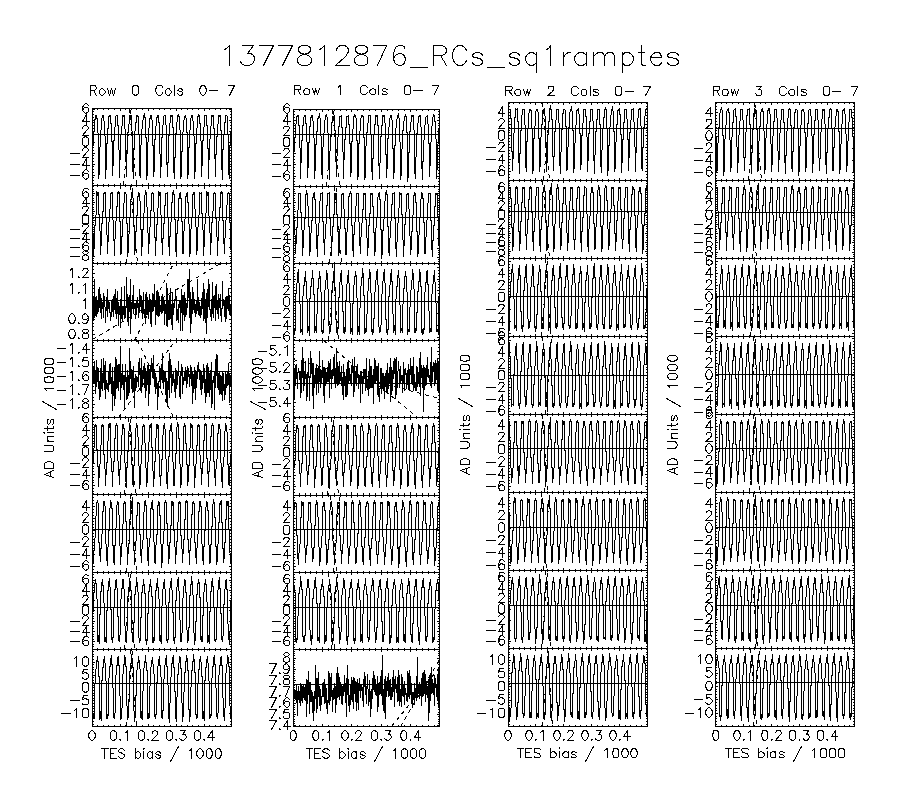
\includegraphics[width=\textwidth]{./images/1377812876_RCs_sq1ramptes_00.png}
\caption{Plot showing response of SQUID amplifier chain to ramp in \TES\ bias current, while \TES\ is superconducting. Data is shown for rows 0--4 for all eight columns. \RC{0}{2}, \RC{0}{3}, \RC{1}{3}, \RC{1}{7} all show no response, only noise (note the change in vertical scale for these row/columns). xxx need to explain units on axes?}
\label{fig:tes-bias-ramp-sc}
\end{figure*}

\begin{figure*}[th]
\centering
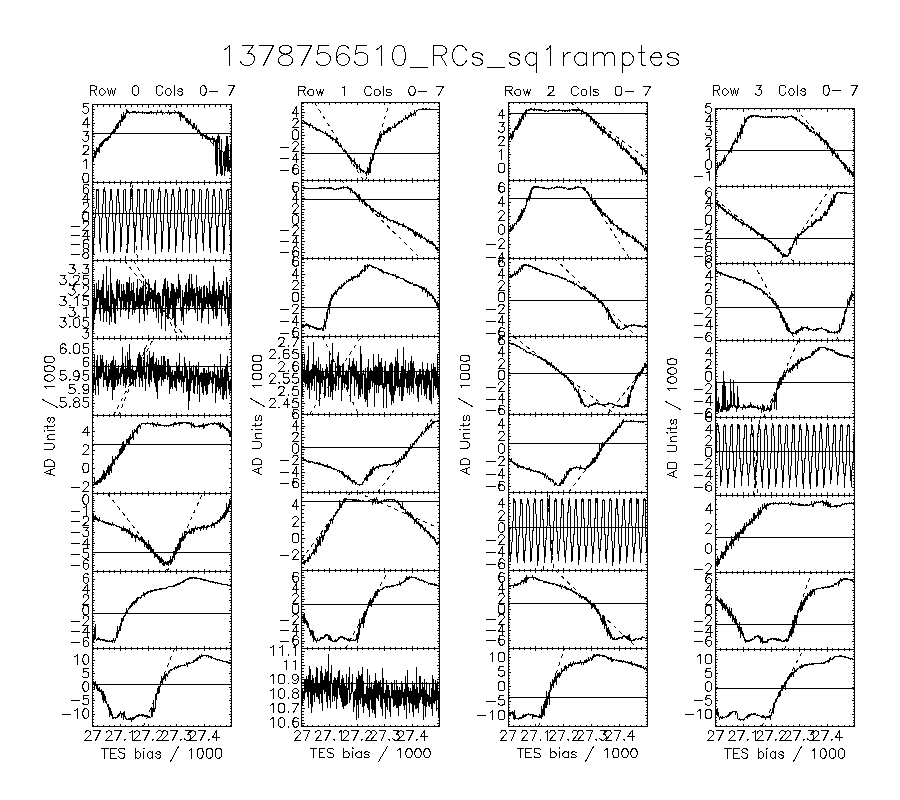
\includegraphics[width=\textwidth]{./images/1378756510_RCs_sq1ramptes_00.png}
\caption{Plot showing response of SQUID amplifier chain to ramp in \TES\ bias current, while \TES\ is biased into transition. The change in applied bias current is the same as in \figref{fig:tes-bias-ramp-sc}.
Data is shown for rows 0--4 for all eight columns.
\RC{0}{2}, \RC{0}{3}, \RC{1}{3}, \RC{1}{7} all show no response, only noise (note the change in vertical scale for these row/columns).
\RC{0}{1}, \RC{2}{5} and \RC{3}{4} all respond as if they were still superconducting (see \figref{fig:tes-bias-ramp-sc}).
The much slower mapping of the $V$-$\phi$ curve indicates a much higher resistance in the \TES\ circuit loop, due to the \TES\ itself starting to go normal.
xxx need to explain units on axes?}
\label{fig:tes-bias-ramp-trans}
\end{figure*}

\begin{figure*}
\centering
\includegraphics{./drawings/ch8-detector-cuts-wafer.pdf}
\caption{
Figure showing detector layout, highlighting which detectors have problems and which are working.
Each detector is labeled (below) with its row/column.
The x and y positions of the detectors on the wafer are also given, given in this thesis in the format X-Y, where X give the x position of the detector (labeled along the bottom) and Y the y position (labeled along the left).
}
\label{fig:detector-cuts-wafer}
\end{figure*}

\begin{figure*}
\centering
\includegraphics{./drawings/ch8-detector-cuts-rc.pdf}
\caption{Figure showing same information as \figref{fig:detector-cuts-wafer}, but organized in term of readout rows/columns. Each detector is labeled (below) with its position on the detector wafer. The rows/columns are labeled on the left and top. Unused row/columns as well as the row/columns used to readout the position of the secondary mirror are also indicated. }
\label{fig:detector-cuts-rc}
\end{figure*}

\section{Readout of Mirror Position}\label{sec:ch8-mirror-readout}

The \Imager\ produces a time-ordered data stream containing the output of each detector as a function of time.
In order to turn this data stream into a video, we must know where the optical system is pointing at all times.
This section desribed how this pointing information is placed directly into the timestream by the \Imager.
It is also necessary to know where each detector is pointed relative to the optical system; this relative detector pointing information is extracted from beam maps, as discussed in \sectionref{s:beam-maps}.

The pointing of the optical system is set by the positions of the two actuators --- \DISP1 and \DISP2 --- that move the secondary mirror.
The actuator control hardware provides two voltage signal which are proportional to the positions of the actuators.
This voltage signal is sent into the \Imager\ cryostat by a pair coaxial cables.
Inside the cryostat two \SI{1}{m} long Phosphur Bronze (xxx exact lakeshore name?) (PhBr) \AWG36 twisted pair wires carry the signal to the focal plane, where the signal is fed into the input coil of a 1st stage \SQUID.
Series resistors (\SI{4.23}{\mega\ohm} for \DISP1, \SI{4.36}{\mega\ohm} for \DISP2) are used at room temperature to reduce the maximum current flowing through the wires to a value appropriate for the 1st stage \SQUID\ input; approximately \SI{2}{\uA}.

This approach synchronizes the actuator position readout with the detector response, and allows both pieces of information to be readout in the same way.

To convert the mirror output current (readout as en electrical current by the readout system) to actuator displacement I moved the mirror actuators in sine-wave patterns with a frequency of \SI{0.1}{\Hz} using 8 different displacement ampitudes.
I fit the resulting output current timestream to a sine waves.
The result are conversion factors of \SI{2.929}{\mm\per\uA} for \DISP1 and \SI{3.024}{\mm\per\uA} for \DISP2.
% see cooldown39/ana_bose_factor.m

% xxx
% I think the way to handle my distance-scale discrepancy is to
% explicitly introduce a fudge-factor here, and state that
% measuremnets in section whatever show that this value is foo.
%
% Then the big mystery becomes the grid spacing on the detector focal
% plane. Unfortunately I don't have anything to say about what's going
% on with this, but that's the way that it is!
To convert actuator displacement to displacements in the farfield of the system, I used the conversion factors produced from \ZEMAX\ listed in \sectionref{sec:ch4-optical-design}.
A \SI{1}{\mm} movement of the actuator produces a change in angle of the secondary mirror of \ang{0.276}; a \ang{1.0} rotation of the secondary mirror displaces the beam of an on-axis detector by \SI{18.35}{\cm} at the far-field focal plane.
The conversion factor between actuator displacement and farfield beam displacement is \SI{5.065}{\cm\per\mm}.

To convert actuator displacements into locations in the farfield, three additional factors should be considered.
First, the cassegrain optical system inverts images that it views, so that a beam from a detector in the lower left of the focal plane (as viewed from behind the detector focal plane) is pointed to the upper right on the farfield image (again as viewed from the system).
Second, tilting the mirror displaces the beams in the same direction as the mirror is tilted; this is easily seen by thinking of the system in transmission, and imagining the way a beam of light is reflected off of a rotated mirror).
Third, the actuators are oriented so that their rotation axes are rotated from horizontal/vertical by \ang{45}.
This all means that --- as viewed from the cryostat --- positive displacements of the \DISP1 actuator shift beams up and to the right, while positive displacements of the \DISP2 actuator shift beams up and to the left.
If we consider an $x$-$y$ coordinate system in the farfield, this means that the $x$ and $y$ displacement of the beams due to mirror movements are calculated as
\begin{equation}
\Delta x = F_d \frac{\sqrt{2}}{2} \left( I_{\DISP1} \times \frac{\SI{2.929}{\mm}}{\SI{1}{\uA}} -
                              I_{\DISP2} \times \frac{\SI{3.024}{\mm}}{\SI{1}{\uA}}  \right) \times
    \frac{\ang{0.276}} {\SI{1}{\mm}} \times
    \frac{\SI{18.35}{\cm}} {\ang{1}}
\end{equation}
\begin{equation}
\Delta y = F_d \frac{\sqrt{2}}{2} \left( I_{\DISP1} \times \frac{\SI{2.929}{\mm}}{\SI{1}{\uA}} +
                              I_{\DISP2} \times \frac{\SI{3.024}{\mm}}{\SI{1}{\uA}}  \right) \times
    \frac{\ang{0.276}} {\SI{1}{\mm}} \times
    \frac{\SI{18.35}{\cm}} {\ang{1}}
\end{equation}

Here I have also introduced a ``fudge factor'' $F_d$, which allows us to account for any error in manufacturing of the optics, errors in the \ZEMAX\ model, or errors in the \BOSE\ actuator control system; e.g., when we tell the \BOSE\ system to move an actuator by \SI{3}{\mm}, does it really move exactly \SI{3}{\mm}?
If none of these --- or other --- errors are present in the system, then $F_d$ will be equal to 1.0.
The direct measurements of distances in the farfield described in \sectionref{xxx} show that $F_d = 1.16$, and this value is used in all analysis for the remainder of this chapter.

% pivot 14.19 mm behind mirror vertex
% pivot 14mm in front on \BOSE\ attachment point

A natural question is whether cross-talk appears between the actuator readout and the other detectors.
To test this both actuators were moved in a \SI{6}{\Hz} sine-wave pattern over their maximum displacement range of +/- 3.5~mm, while the detectors were bias at \SOC.
Both actuators were moved at the same time, roughly \SI{135}{\degree} out of phase.
The level of crosstalk present can be quantified by performing a least-squares fit of each detector timestream $\vect{d}_{rc}$ to the model
\begin{equation}
	 \vect{d}_{rc} = A_1 \vect{d}_{\DISP1} + A_2 \vect{d}_{\DISP2}.
\end{equation}
Here $\vect{d}_{\DISP1}$ and $\vect{d}_{\DISP2}$ are the measured outputs for each actuator.

To check whether crosstalk from the actuators is a problem for our system, I calculated the crosstalk amplitudes $A_1$ and $A_2$ for each detector twice: once of the first half of the data acquision and once for the second half.
If crosstalk is present to a statistically significant level, a scatterplot of the crosstalk amplitudes for the two halfs of the data acquisition should show signs of correlation.
As can be seen in \figref{fig:ch9-bose-cross}, the points are clustered about the origin, indicating no consistent crosstalk amplitude, and no correlation is apparent.

\begin{figure*}[th]
\centering
\includegraphics[width=\textwidth]{drawings/ch8-bose-cross.pdf}
\caption{
Plot showing crosstalk amplitudes.
The left plot is for \DISP1, the right for \DISP2.
Each actuator was moved +/- \SI{3.5}{\mm} at 6 Hz while the detectors were biased at \SOC.
The best-fit crosstalk amplitude for each actuator and detector were calculated for both the first half and the second half of the data acquisition, and these amplitudes are plotted against each other in these plots.
The lack of correlation in the scatter plots, as well as the clustering around the origin, indicates that any crosstalk present cannot be distinguished from noise in the detectors.
}
\label{fig:ch8-bose-cross}
\end{figure*}

% xxx - I get 500 uW for the load from these four wires (300 K - 1K). Can this be correct? I'm sure I did this calculation in the past and got a much smaller number. Did I screw up in the past? Is today's calculation in error? Am I intercepting this load at 50~K or 4~K, and I forgot about that? Did I use a much longer wire than 1~m? This could be a big cryogenic problem!

\section{Focus Distance}\label{s:focus-distance}

As described in \sectionref{s:optical-design}, the \Imager\ is designed to focus at distances of 16~m -- 30~m (xxx check 2nd distance).
All results described in this chapter were with the \Imager\ configured to focus at 16~m.
To check the actual distance to the target focal plane, beam maps as described in \sectionref{s:beam-maps} were performed with the blackbody source located at different distance from the cryostat.
\figref{fig:beam-vs-distance} shows beam maps for the same detector taken at different distances.
It is clear from this plot that the best focus occurs at \abt{\SI{17}{m}}, and the depth-of-field is approximately xxx~m.

The reasons for the difference from \ZEMAX\ predictions are not understood.
Possibilities include the cryostat being located too close to the primary mirror and the primary (or secondary) mirrors having an incorrect shape.

\section{Beam Maps} \label{sec:ch8-beam-maps}

As discussed in \sectionref{sec:ch4-feedhorn-design}, the \Imager\ feedhorns are predicted to have beams that are circularly symmetric and well-approximated by Gaussians with \FWHM\ of x.xx~cm at the target.
To verify these predictions beam maps were performed by rastering the beams over a small, stationary \SI{1030}{\celsius} blackbody source.

The blackbody source used was an IR Labs xxx\footnote{IRLabs, Inc. Tucson, AZ. USA}.
This source reaches a maximum of \SI{1030}{\celsius} and has apertures ranging in size from x.xx in to x.xx in.
Best results were achieved by covering an area around the blackbody source with Aluminum foil; this eliminated hotspots in the image due to the warmth of the housing of the blackbody source itself.
\figref{xxx} shows a picture of the blackbody source with Aluminum foil mask.

The \Imager\ beams were rastered over the blackbody source by moving one actuator at \SI{6}{\hertz} while the other actuator moved much more slowly at \SI{0.1}{\hertz}.
Scans were taken with the blackbody in two different locations to ensure coverage of the entire subarray.
At each blackbody positions two scans were taken with \DISP1 as the fast actuator and two with \DISP2 as the fast actuator, for a total of eight scans.

For each scan, the data stream for each detector was ``binned'' as described in \sectionref{xxx} to produce a beam map for each detector.
No common mode or polynomial was removed from the timestreams.
Actuator displacements were converted to distances in the far-field using the conversion factors discusssed in \sectionref{sec:ch8-mirror-readout}.
The following 2-D Gaussian allowing for ellipticity was then fit to each beam map:
\begin{multline}
%\begin{split}
  P(x,y) = O + A \exp{ \left[  - \frac{1}{2} \left( \frac{ (x-x_0) \cos{\theta} + (y-y_0) \sin{\theta}}{\sigma_1} \right)^2 
                               - \frac{1}{2} \left( \frac{-(x-x_0) \sin{\theta} + (y-y_0) \cos{\theta}}{\sigma_2} \right)^2
                       \right] }.
%\end{split}
\end{multline}
Here $x$ and $y$ represent the position in the beam map, while $x_0$, $y_0$, $\sigma_1$, $\sigma_2$, $\theta$, $A$, and $O$ are the parameters to be fit.
$O$ represents an overall \DC\ offset in the map level.
Only the points within \SI{3}{\cm} of the map peak were included in the fit.
Beam maps at the edge of the scan were discared, as were beam maps where the fitting routine performed poorly.
The $\theta$, $\sigma_1$, and $\sigma_2$ paremeters were all rationalized so that the conditions $\sigma_1 > \sigma_2$ and $0 < \theta < \ang{180}$ hold.
The beam parmeter across the eight scans were then averaged together to produce final beam maps.
\figref{fig:ch8-beam-summary} summarizes the final fit parameters for all the beams.
The beam ellipticity and angle offset from the $x$-axis are statistically significant.

\figref{fig:ch8-all-beam-maps} shows the final beam maps.
The beams are elliptical, with a mean $\sigma_1 / \sigma_2 = \si{1.6}$.
The mean beam angle is $\ang{70}$ from the $x$-axis.
The beam size \FWHM\ is \SI{1.4}{\cm}, and is calculated from
\begin{equation}
  2 \sqrt{2 \ln{2}} \sqrt{\sigma_1 \sigma_2}
\end{equation}
where the prefactor $2 \sqrt{2 \ln{2}}$ converts from the Gaussian parameters $\sigma$ to the gaussian \FWHM.

In \sectionref{sec:ch4-feedhorn-design}, it was shown that the expected \FWHM\ beam width from this measurement is \SI{1.18}{\cm}, about \SI{19}{\percent} smaller than observed.
The beams should also be circular rather than strongly elliptical as observed.
The source of the large beams and ellipticity is not known, but three possible explanations are (1) misalignment of the feedhorns with the primary and secondary mirrors (2) diffraction off the aperture stop located in the \SI{50}{\kelvin} radiation sheild (3) errors in fabrication of the mirrors or feedhorns.

The best-fit grid spacing between detector beams in the far field is \SI{2.0}{\cm}.
Using the plate scale extracted from \ZEMAX\ in \sectionref{sec:ch4-optical-design}, this is equivalent to a \SI{3.2}{\mm} detector spacing on the focal plane array.
The design detector spacing, after accounting for predicted thermal contraction of the feedhorn arrays, was \SI{2.730}{\mm}, \SI{15}{\percent} smaller than this.
Although the ellipticity of the beams is disappointing, the resolution is close to target, and the ellipticity is not a barrier to using the system to take video images. The next section describes the algorithm use to turn detector timestreams into videos.

\begin{figure*}[th]
\centering
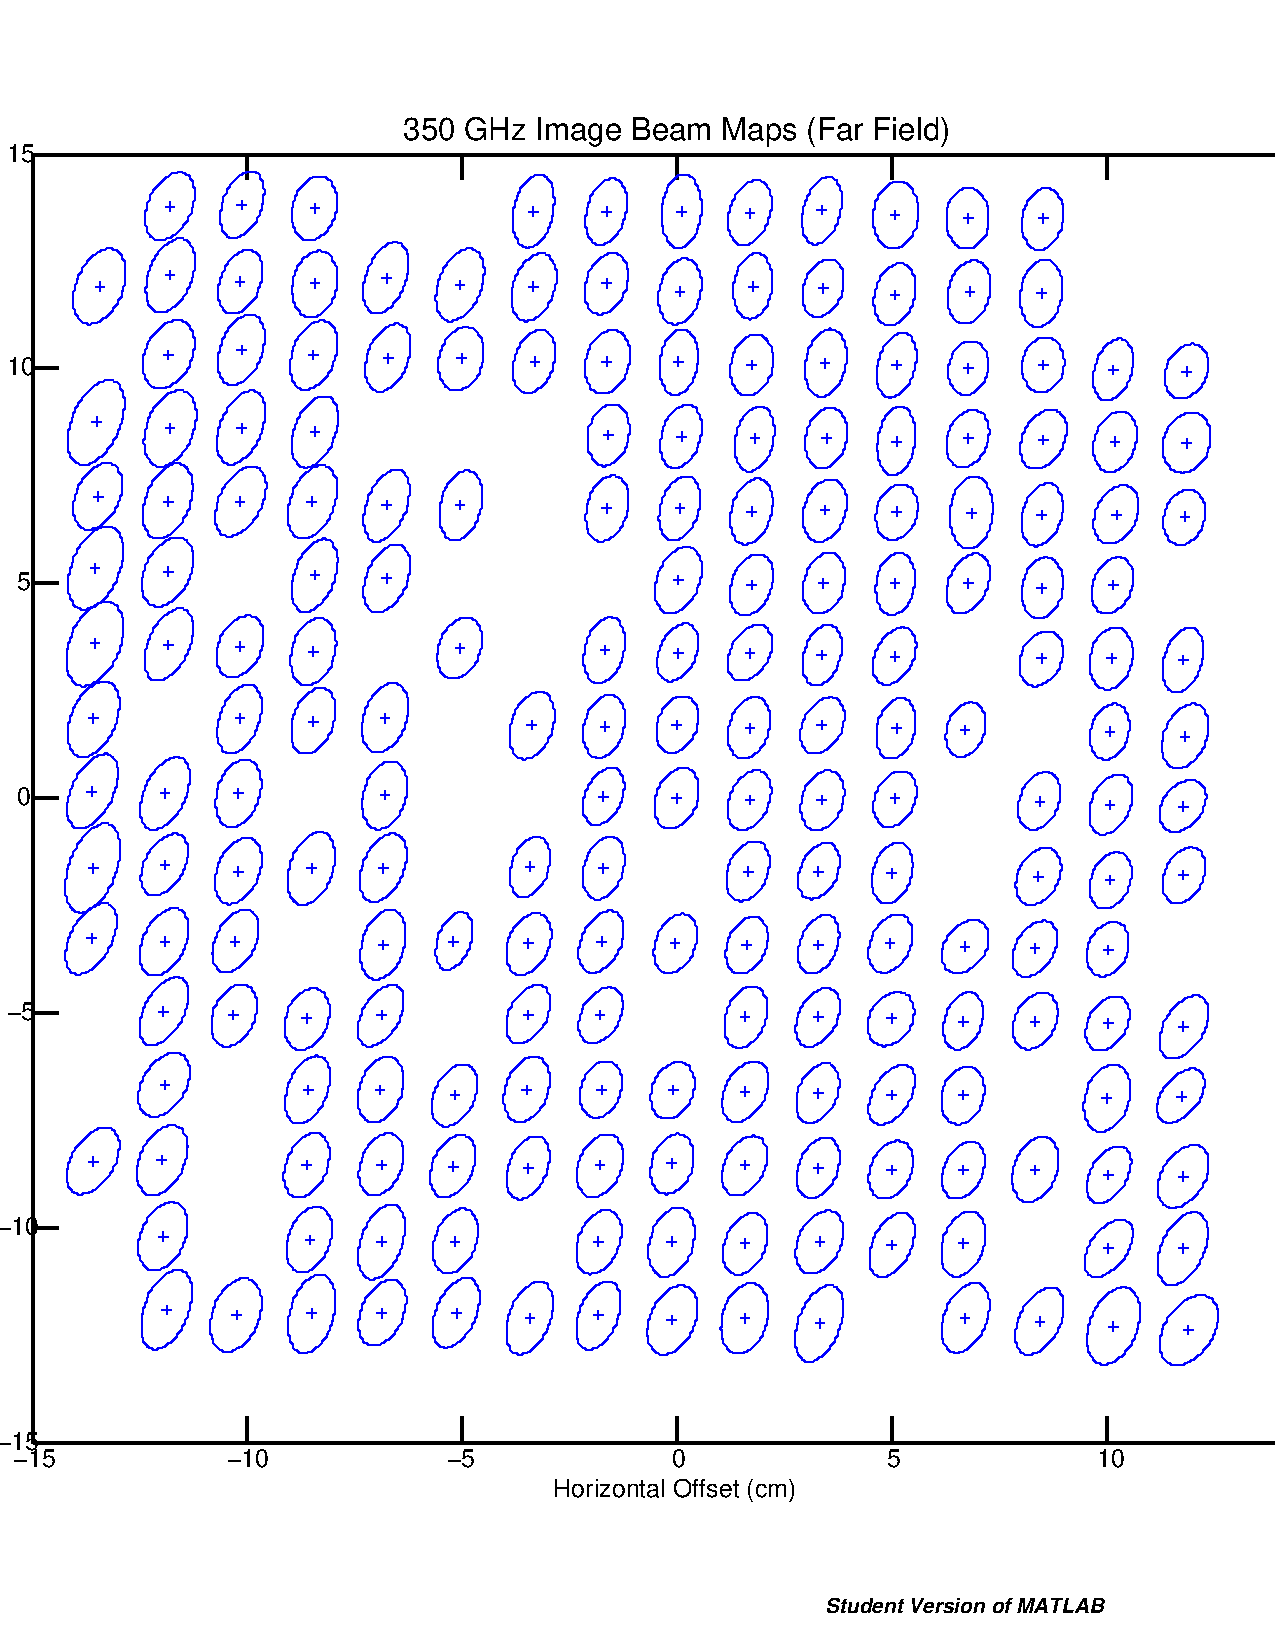
\includegraphics[width=\textwidth]{drawings/ch8-all-beam-maps.pdf}
\caption{
Plot showing final beam maps.
The ellipses represent the full-width-half-maximum of the best-fit 2-D Gaussian for each beam. The beams are elliptical, with a mean $\sigma_1/\sigma_2$ of 1.6, mean beam angle to the $x$-axis of \ang{70}, and beam FWHM of \SI{1.4}{\cm}.
The four grid locations in the extreme upper right corner, as well as the extreme lower left grid point, have no detectors and therefore no beams. All other missing beams are for cut detectors, as discussed in \sectionref{sec:ch8-det-cuts}.
The offset is relative to detector \RCm{18}{4}.
}
\label{fig:ch8-all-beam-maps}
\end{figure*}

\begin{figure*}[th]
\centering
\includegraphics{drawings/ch8-beam-summary.pdf}
\caption{
  Plots summarizing final fit parameters for all beams.
  \textbf{Left Column} Histograms of beam \FWHM\ (defined in text), beam ellipticity (defined as $\sigma_1 / \sigma_2$) and beam angle to $x$-axis.
  \textbf{Right Column} Scatter plots showing correlation of the three parameters with each other. Beam \FWHM\ increases with ellipticity; this is to be expected give it's definition.
}
\label{fig:ch8-beam-summary}
\end{figure*}

\section{Direct Measurement of Distance Scale} \label{sec:ch8-dist-scale}

To measure the factor $F_d$ described in \sectionref{sec:ch8-mirror-readout}, I placed a styrofoam cooler filled with liquid Nitrogen (LN2) in the farfield of the system and scanned the system over it, using data acquired to create still images.
A sheet of Eccosorb xxx was placed in the cooler to serve as a cold black surface for the system to observe.
Images were acquired of the cooler itself, as well as the cooler with aluminum foils strips taped to the outside.
Each strip was \abt{\SI{4}{\cm}} tall, and the strips were \SI{14.5}{\cm}, \SI{29}{\cm}, and \SI{47.2}{\cm} long.
The interior of the cooler is \SI{67.7}{\cm} wide.
For each image the \FWHM width of the strip --- or the cold space inside the cooler --- was calculated by taking a cut through the still image centered n the strip or cooler.

The result of these measurements is that $F_d = 1.16$.
The source of this discrepancy is not understood.

% xxx might be nice to have plots for this section, but need to move
% on for now.

% Code: imaging/ana_reso_from_stills.m

\section{Direct Measurement of Resolution}

Using the same cooler filled with LN2 described in \sectionref{sec:ch8-dist-scale}, a dime (diamter \SI{17.91}{\mm}) was taped to the outside of the cooler and a still image was taken.
\figref{fig:xxx} shows the resulting still image, as well as a close-up of the are with the dime.
A 2-D Gaussian was fit to resulting map.
The best-fit Gaussian has ellipticity 1.16 --- smaller than the individual beams, as expected due to convolution with the dime, which is not a point source.
The \FWHM\ of the dime map is \SI{2.0}{\cm}; a bit larger than the dime's width of \SI{1.791}{\cm}, as expected due to convolving with the beam.
This serves as a rough confirmation of the beam size and locations as determined in \sectionref{sec:ch8-beam-maps}.

\begin{figure*}[th]
\centering
\includegraphics{drawings/ch8-dime-map.pdf}
\caption{
  Plots showing still image of cooler filled with LN2, with a dime (diameter \SI{1.791}{\cm}) taped to it's outside.
  Red is warm, blue cold; the temperature scales are different in the two plots.
  \textbf{Left} The full map of the cooler. The white rectangle shows the area of the detail on the right.
  \textbf{Right} Detail of area within white rectangle: the dime.
  The black ellipse shows the \FWHM of the best-fit ellipse to the map. The ellipticity is \num{1.16}, the FHWM of the principal axes are \SI{1.83}{\cm} and \SI{2.12}{\cm}, for an overall \FWHM\ of $\sqrt{1.83 \times 2.12} = \SI{2.0}{\cm}$.
}
\label{fig:ch8-dime-map}
\end{figure*}

\section{Optical Efficiency} \label{sec:ch8-opt-eff}

To measure the total optical efficiency of the system, \IV\ curves can be taken while a detector's beam is pointing at two known temperature distributions.
As discussed in \sectionref{xxx}, the different in Joule power at $0.99 R_n$ gives the difference in power absorbed in the bolometer.
If the two temperatures are $T_1$ and $T_2$, then the total optical efficiency $\eta_{tot}$ is given by
\begin{equation}
  \eta_{tot} = \frac{P_{iv,1} - P_{iv,2}}{P_{opt}(T_2) - P_{opt}(T_2)},
\end{equation}
where $P_{IV}$ is the Joule power in the detector at $0.99 R_n$ and $P_{opt}(T)$ is the optical power in both polarizations emitted by the source in a single spatial mode, given by \eqnref{xxx}.

For a good measurement the two temperatures $T_1$ and $T_2$ should be as far apart as possible, and the detector's farfield beam should be filled by the tmperature distribution in each case.
I used the same ``eccosorb submerged in LN2'' setup as described in \sectionref{xxx} for the cold temperature.
For the warm tempearute I used a sheet of AN72 Eccosorb backed by a thin sheet of Aluminum.
``Room Temperature'' here is assumed to be \SI{295}{\kelvin} (\SI{71.3}{\fahrenheit}).
Although the temperature of LN2 is welll known to be \SI{77}{\kelvin}, this does not mean that the temperature seen by the beams when pointed at the cooler is exactly \SI{77}{\kelvin}.
The beams are looking through the \SI{1.625}{\in} thick styrofoam walls of the cooler, which may have some emission themselves.
Although the eccosorb sunk in LN2 transmits no power at \SI{350}{\GHz}, it may reflect some amount of light from the surrounding room.
It is possible that a small amount of water vapor could condense on the outside of the cooler, leading to further emission.
For the purposes of this measurement I assumed that the eccosorb was totally black and sitting at \SI{77}{\kelvin}.
I also assume that no water vapor was condensed on the cooler, which is consistent with a visual examination.
I assume a non-unity transmittivity $\tau$ for the styrofoam.

For each of eight detectors, four IV curves were taken under three conditions: pointing at the room-temperature eccosorb, pointing at the cold eccosorb in the cooler, and looking at the eccorb with the cooler's lid placed directly in front of the cooler.
The lid is \SI{2}{\in} thick and the cooler's side is \SI{1.625}{\in} thick.
I assume that the tranmitivity takes the form $e^{-t \kappa}$, where $t$ is the thickness of the material and $\kappa$ is some constant which characterizes the attenuation length of \SI{350}{\GHz} light in styrofoam.
Given this assumption, if the transmissivity through the cooler's wall is $\tau$, then the transmittivity through the lid is given by $tau^{2/1.625} = \tau^{1.23}$.

The optical powers viewed under these three conditions is then given by
\begin{equation}
  P_{opt,ecco} = P_{opt}(T_h)
\end{equation}
\begin{equation}
  P_{opt,LN2} = \tau P_{opt}(T_c) + (1-\tau)P_{opt}(T_h) = P_{opt}(T_h) - \tau (P_{opt}(T_h) - P_{opt}(T_c)),
\end{equation}
\begin{equation}
  P_{opt,LN2,lid} = \tau^{1.23} P_{opt,LN2} + (1-\tau^{1.23})P_{opt}(T_h) = P_{opt}(T_h) - \tau^{2.23}(P_{opt}(T_h) - P_{opt}(T_c)) .
\end{equation}
The differences in optical power absorbed in the bolometer will then be
\begin{equation}
  \Delta P_{b,ecco,LN2} = \eta \tau (P_{opt}(T_h) - P_{opt}(T_c)),
\end{equation}
and
\begin{equation}
  \Delta P_{b,lid,no lid} = \eta \tau (1-\tau^{1.23}) (P_{opt}(T_h) - P_{opt}(T_c)).
\end{equation}
These last two equations can be solved for $\eta$ and $\tau$. The results are
\begin{equation}
   \tau = \sqrt[1.23]{1 - \frac{\Delta P_{b,lid,no lid}}{\Delta P_{b,ecco,LN2}}},
\end{equation}
\begin{equation}
   \eta = \frac{\Delta P_{b,ecco,LN2}}{ \tau ( P_{opt}(T_h) - P_{opt}(T_c) )} .
\end{equation}

The above sets of three \IV\ curves were repeated three times over the course of several hours.
\tableref{tab:opt-eff} gives the results of these measurements averaged over all detectors and all repetitions.
The transmitivitty $\tau$ of the cooler wall was found to be \abt{\SI{90}{\percent}} and the optical efficiency $\eta_{tot}$ was \SI{13.6}{\percent}. 

This optical efficiency is roughly half of the value predicted in \sectionref{xxx}.
It it not clear where the optical power is being lost.
As a rough check I took \IV\ curves when the cryostat window was covered with aluminum foil.
In this condition no light from outside the cryostat can reach the detectors.
The result was that \SI{38.6}{\pW} less power was falling on the detector, a further decrease of \SI{13}{\pW} from when the beams are pointed at LN2.
It is difficult to interpret this measurement because it is not clear what temperature distribution the detectors are now seeing.
% xxx should I just remove this because of difficulty of interpretation?

\begin{table*}[t]
\centering
\caption{
Results of optical efficiency measurments.
The values are medians and the uncertainties give the \SIrange{25}{75}{\percent} range of measured values.
}
\label{tab:opt-eff}
\begin{tabular}{l l}
\toprule
Quantity &  Value \\
\midrule
$\eta$ & $13.6 \pm  0.9$ \% \\ 
$\tau$ & $90.6 \pm  4.8$ \% \\ 
$P_{b,ecco,LN2}$   & $25.6 \pm  0.5$ pW \\ 
$P_{b,lid,no lid}$ & $ 2.0 \pm  1.0$ pW \\
\bottomrule
\end{tabular}
\end{table*}
 
\section{Establishment of Temperature Scale} \label{sec:ch8-temp-scale}

The output of the readout system gives changes in current passing through the detectors.
In order to change this current change to a temperature change we must first convert the current changes to power changes by dividing by the power-to-current responsivity $s_I$.
These power changes are in terms of power absorbed in the bolometer.
To convert to temperatures changes in the farfield of the system, we must use the total optical efficiency $\eta_{tot}$, as well as the Raleigh-Jeans limit of the optical power per spatial mode from a temperature distribution (see \sectionref{xxx}).
The result is that the conversion from current to temperature is given by
\begin{equation} \label{eqn:ch8-I-to-T}
  \Delta T = \frac{\Delta I}{s_I(0) 2 k_B \eta_{tot} \Delta \nu}.
\end{equation}

Ideally this temperature scale would be measured directly by allowing the detectors to observe two known temperature distributions and measuring the resulting change in current.
However, this is easier said than done.
As the amount of optical power absorbed in a detector changes, the point occupied by the detector on its $R(T,I)$ surface changes, so that \Loop\, $\beta_I$, and the bias voltage $V_0$ all change.
This leads to a changing responsivity with optical load through \eqnref{xxx}.
For small changes in load (such as we expect in images taken with the system) the changes will be small and can be ignored.
But in order to obtain an accurate measurement of the temperature scale, it is desireable to use a large change in temperature, such as the difference between room temperature and LN2.
For these larger temperature changes the change in responsivity may not be negligible. 

To check the order of magnitude of this effect, I measured the detector responsivity directly using heaters both when the system was observing eccosorb and when the cryostat window was covered with aluminum foil.
Covering the window with foil reducing the optical power reaching the detectors from outside the cryostat by \abt{\SI{38}{\pW}}.
For two of the detectors this lead to an increase in responsivity of \abt{\SI{1}{\percent}}, for the other two the increase was \abt{\SI{6.5}{\percent}}.
This makes using LN2 to establish a temperature scale that is more accurate than \abt{\SI{10}{\percent}} challenging.

Changing responsivity would not be a problem if the two temperatures were close to both each other and room temperature.
Stable, uniform temperature distributions using stirred liquid water are avalable \cite{grossman h20 standard} and should be used if a more accurate temperature mapping is desired in the future.

For this thesis, however, I have not made these measurements.
Instead I have assumed that all detectors have the same optical efficiency as was measured for eight detectors in \sectionref{sec:ch8-opt-eff}, $\eta_{tot} = 0.136$.
For $s_I(0)$ I have use the predicted values at \SOC\ of \sectionref{sec:bias-step}, with the exception of three detectors (\RCm{25}{4}, \RCm{26}{2}, \RCm{26}{4}) for which the predicted $s_I(0)$ was clearly incorrect, as judged from looking at detector timestreams and still images.
For these three images I have assumed a responsivity equal to the mean of all other predicted responsivities.

As a check on the accuracy of this temperature scale, the still image on the left of \figref{fig:ch8-dime-map} has \abt{\SI{180}{\K}} of contrast between the coldest section at the middle of the cooler and the warm area to the left of the cooler.
Given our estimate of transmittivity $\tau$ of the cooler walls of \num{0.9}, the expected temperature differential is $0.9(295-77) = \SI{196}{\K}$.
Given the fact that responsivity will increase with optical loading, which leading to underestimates of temperature difference via \eqnref{eqn:ch8-I-to-T}, these numbers are fairly close.

From this I conclude that while the temperature scale is likely not accurate to withing \SI{5}{\percent}, it is probably correct to within \SI{20}{\percent}.

\section{Image Processing Algorithm} \label{sec:ch8-algo}

This section describes the algorithm used to turn raw detector timestreams into video images.
The algorithm currently used is very simple, and processes one video frame at a time.

The algorithm steps are as follows:
\begin{enumerate}
\item The  \MCE\ channles containing the actuator displacement (\RCm{32}{5} for \DISP1 and \RCm{32}{6} for \DISP2) are converted to displacements in the farfield as described in \sectionref{sec:ch8-mirror-readout}.
\item Each detectors output is normalized by dividing it by the amplitude of the best-fit guassian from the beam mappings. This accounts for differences in responsivity as well as optical efficiency between detectors. At this point the units for all detector timestreams should be the same, but each detector timestream will have some unknown offset.xxx need to cover this earlier - maybe an optical efficiency section?
\item Determine full range of farfield positions pointed to, accounting for all detectors. Define a \SI{1}{\cm} grid that covers this range in both $x$ and $y$ directions.
\item Divide detector timestreams into sections for each video frame based on \MCE\ readout rate and frequency at which the secondary mirror is rotating.
  If the mirror frequency is $f_m$ and the readout frequency is $f_{ro}$, then each video frame will cover $\lceil f_{ro} / f_{m} \rceil$.
  \textbf{Example:} If the readout frequency is \SI{3125}{\Hz} and the mirror frequency is \SI{6}{\Hz}, then each video frame will cover $\lceil 520.83 \rceil = 521$ samples.
\item For each video frame
  \begin{enumerate}
  \item Perform the following processing for each detector that is not on the cut list described in \sectionref{sec:ch8-det-cuts}:
    \begin{enumerate}
    \item If the detector's timestream shows evidence of glitches, do not include that detector's timestream for this video frame. The simply algorithm used to identify glitches is the following:
      \begin{enumerate}
      \item Calculate the differences between each consequtive value in the timestream.
        If the timestream values are $f_j$, then the differences are $\Delta f_j = f_{j+1} - f_j$.
      \item Calculate the standard deviation of the differences $\Delta f_j$.
      \item If the absolute value of any $\Delta f_j$ is greater than five times the standard deviation, identify this detector as having a glitch, as so to be ignored for this video frame. xxx should say how often this happens, show example of glitch timestream ... maybe show a big plot with all timestreams for a frame, highlighting those with glitches?
      \end{enumerate}
    \item Subtract the median value for this video frame's detector timestream.
          Although crude, this approach does a good job of accounting for the offsets in the detector timestreams, as well as accounting for the common-mode drift described in \sectionref{sec:common-mode}.
    \item If the detector does not have a glitch, determine which image pixel the detector is pointing to at each point in time, using both the pointing position from the actuator readout described in \sectionref{sec:ch8-mirror-readout} and the beam pointing information from \sectionref{sec:ch8-beam-maps}.
    \item Add the detector's value to that pixel for the frame
    \item Keep track of the total number of pixels that have been aded to each pixel
    \end{enumerate}
  \item After each detector has been processed for the frame, divide the value for each pixel by the number of detector that have been used for that pixel
  \end{enumerate}
  \item To improve constrast, all temperature offset values below xxx K are mapped to xxx K, and all temperature values above xxx K were mapped to xxx K.
        Any pixels in the image with no data were assigned a temperature of xxx K.
  \item After all video frames have been processed, convert the resulting 3-dimensional array to a video using \MATLAB's \texttt{VideoWriter} object.
\end{enumerate}

\figref{fig:ch8-single-frames} shows four still images from a vide that was processed according to these rules.
They show the author with a ceramic knife hidden beneath a button-down cotton shirt.
The ceramic knife is visible as a dark area on the left of the shirt.
A darker line running down the center of the shirt is due to the extra layer of cotton backing the buttons; this additional cloth produces more attenuation of the warm light from the body, and so appears cooler.

xxx need to give a URL to where this particular video can be viewed.

xxx need to comment on temperature scale in this image!

\begin{figure*}[th]
\centering
\includegraphics[width=\textwidth]{drawings/ch8-single-frames.pdf}
\caption{
Sample still images from a video taken with the \Imager.
Time proceeds left-to-right and top-to-bottom.
The stills are 20 frames (\SI{3.33}{\s}) apart.
The person in the images is the author.
A ceramic knife hidden beneath a button-down cotton shirt is visible on the left of each image.
The darker line running down the center of the shirt is due to the extra layer of cotton backing the buttons; this additional cloth produces more attenuation of the warm light from the body.
xxx say something about temperature scale once I get it right.}
\label{fig:ch8-single-frames}
\end{figure*}

\section{Image Noise Model}

The temperature scale established in \sectionref{sec:ch8-temp-scale} allows us to convert the measured detector white-noise level of \abt{\Pnoise{2.4e-15}} to a temperature noise via
\begin{equation}
  S_T = \frac{S_P(0)}{2 k_B \eta_{tot} \Delta \nu}.
\end{equation}
This results in a temperature noise level of \abt{\Tnoise{15e-3}}, referred to the temperature viewed in the farfield of the system.

To use this noise level to make a prediction for the \NETD\ in the image we can use the radiometer equation \cite{dicke-radiometer}:
\begin{equation} \label{eqn:ch8-radiometer}
  NETD = \frac{S_T}{\sqrt{2 t_{dwell}}},
\end{equation}
where $t_{dwell}$ is the total integration time including all detectors for each pixel in the image.
In this equation the factor of 2 accounts for the fact that the noise power spectral density is defined so that the total variance in the signal is given by the integral of the power spectral density up to the one-half of the sampling frequency, i.e. up to the Nyqust frequency.

All images in this chapter contain \abt{4030} pixels, each \SI{1}{\cm^2} in area%
\footnote{
  Although the images shown are all rectangular, due to the elliptical scanning pattern the actual area of the images that contains data is smaller than the rectangle.
}.
Each video frame lasts \SI{1/6}{\s}, and there are \abt{210} good detector contributing.
$t_{dwell}$ is thus given by
\begin{equation} \label{eqn:ch8-t-dwell}
  t_{dwell} = \frac{210 \times \frac{1}{6}\,\si{s}}{4030} = \SI{8.7}{\ms}.
\end{equation}
Plugging this into \eqnref{eqn:ch8-radiometer} gives an $NETD$ of \abt{\SI{115}{\mK}}.

Verifying this noise level in a video image is difficult because we do not know a-priori whether there are any regions in the image which have a flat temperature distribution.
However, if we place a sheet of eccosorb directly in front of the cryostat window, where all detector beams are large and covering very similar areas, then all detectors should be viewing very close to the same temperature distribution.
If data is acquired in this state, while the secondary mirror is moving, and the resulting timestreams run through the same software used to create ``real'' videos, then the standard deviation of the temperture in each frame should give a god estimate of the NETD.

I carried out this proceedure, creating a ``video'' with 19 frames.
The mean $NETD$ across the 19 frames is \SI{101}{\mK}.
\figref{fig:ch8-flat-netd} shows a histogram of the \NETD\ distribution from all 19 frames, a histogram showing the temperature offset distribution for the second frame (which has $NETD = \SI{100}{\mK}$), the second frame, and one of the still images from \figref{fig:ch8-single-frames}.
Both still images use the same temperature-difference-to-grayscale mapping.

Comparing the two frames visually, it is clear that $NETD$ in the true video frame is dominated not by detector noise, but by artifacts of the scan, visible as elliptical arcs in the image.
These artifacts are likely caused by the median-subtraction scheme of \sectionref{xxx} not properly accounting for the detector offsets.
Nevertheless, in area of the video still where there appear to be few scan artifacts (such as the arem on the lower right), the level of noise in the image appears comparable to the ``flat'' still, indicating that \SI{100}{\mK} is a reasonable estimate of the $NETD$ in the image caused by detector noise.

\begin{figure*}[th]
\centering
\includegraphics[width=\textwidth]{drawings/ch8-flat-netd.pdf}
\caption{
  Plots relating to measurement of \NETD\ in flat frame images.
  \textbf{Upper Left} Histogram of \NETD\ for each of 19 frames taken from a ``flat'' video image. This \NETD\ is defined as the standard deviation of the temperatures across all pixels which were visted by at least one detector. 
  \textbf{Upper Right} Histogram showing distribution of temperature offsets within the second video frame, which has an \NETD\ of \SI{100}{\mK}.
                       The far left and far right bins include outliers that extend all the way to \SI{-1}{\K} on the left and \SI{1.5}{\K} on the right.
                       Removing these outliers results in \NETD\ values that are roughly \SI{15}{\percent} smaller.
  \textbf{Lower Left} The second frame of the flat video.
  \textbf{Lower Right} Frame 25 of the video discussed is \sectionref{xxx}.
These two frames use the same temperature-offset-to-color mapping to aid in visual comparison.
}
\label{fig:ch8-flat-netd}
\end{figure*}

The agreement between the predicted $NETD$ of \SI{115}{\mK} and the observed flat image $NETD$ of \SI{100}{\mK} is an encouraging sign that we understand the behavior of the system.
However, there are several ways in which the noise modelling used in this section simplifies matters:
\begin{itemize}
\item The white noise level for each detector is different.
\item The total integration time per pixel is not uniform. Some pixels end up recieving much more detector samples then others. (xxx quantify)
\item The detector noise is not white.
      \eqnref{eqn:ch8-radiometer} is strictly only true for a noise spectrum that is white, while the detector noise spectrums have rolloffs due to the detector time constant $\tau_{eff}$, \SQUID\ noise, a rolloff due to the \SQUID\ servo loop, and other features.
      Because the noise rolloffs reduce the variance of the detector timestream, this should tend to reduce noise in the map.
      However, the rolloffs also mean that consequtive samples in a detector timestream are correlated, so that averaging them will not reduce noise by the full ``square-root of the number of samples'' factor that is appropriate for uncorrellated noise.
\end{itemize}
A more careful analysis of these factors would be useful, but has not yet been performed.

% Noise can't be reduced very much by sampling much faster than the rolloff in your noise power spectrum.
% But the noise is reduced by a bit, and in this section I quantify that bit.
% An important part of that message is that naively you would think that reducing the number of pixels in an image by a factor of two would reduce noise by a factor of \sqrt{2}, but that in fact because of noise correlations between nearby samples in a detector timestream, the noise reducting will not be that great.

% Noise in our images is reduced by two factors.
% First, each pixel in the image will be visited by more than one detector.
% To the extent that the noise in different detector is uncorrelated --- which is true to a very good approximation at the relevant frequencies of greater then \SI{6}{\Hz} as shown in \sectionref{xxx} --- this effect will reduce noise by the square root of the number of detector which have viewed the pixel.
% Second, each detector may be pointed at a particular pixel for more than one sample.
% If the noise in the detectors was white --- i.e. uncorrelated in time --- than these samples would also reduce noise by the square root f the number of samples.

% Hwoever, as shown in \sectionref{sec:ch7-det-noise}, the detector noise is not white.
% The sampling frequency of \SI{3125}{\Hz} is well above the $\tau_{eff}$ rolloff of the detectors, and close to or above the rolloff of the \SQUID\ servo loop (when $I_{gain}$ is equal to 10 or 20 as is typically for acquiring videos).
% This means that consequtive values in the timestream will be much closer to each other than would be expected by considering the detector white noise level alone, and so the noise will not be reduced as quickly as the square root of the number of samples.

% To account for these factors we consider a detector timestream with values $x_j$ and power spectral density $X^2(f_j)$, defined as
% \begin{equation}
%   X^2_k = \frac{1}{N f_s}
%   \begin{cases}
%     2 |\tilde{x}_k|^2 & 1 \leq k \leq \left\lfloor \frac{N+1}{2} \right\rfloor, \\
%       |\tilde{x}_k|^2 & k = N/2, \text{(only if $n$ is even)}.
%   \end{cases}
% \end{equation}
% Here $\tilde{x}_k$ are the discrete fourier components of the timestream, given by
% \begin{equation} \label{eqn:ch8-dtf-defn}
%   \tilde{x}_k = \sum_{i=0}^{N_1} x_i e^{- 2 \pi j \frac{i k}{N}},
% \end{equation}
% $N$ is the numner of samples in the timestream, and $f_s$ is the sampling frequency.
% The power spectral density is useful because the variance of the timestream is given by\footnote{%
% This can be shown using \eqnref{eqn:ch8-dft-defn}, Parseval's Theorem \cite{xxx} and the fact that the $x_j$ values are all pure real.}
% \begin{equation}
%   \sum_{k=0}^{N-1} Y^2_k \Delta f,
% \end{equation}
% where $\Delta f \equiv 1 / N f_s$.
% Furthermore, it can be shown that convolving the timestream with a kernal $c_n$ results in a new timestream $y_k$ with power spectral density%
%   \footnote{
%     Strictly speaking this result will hold exactly only in the case of a circular convolution.
%     For the case considered here, where the non-zero length of the kernel is much smaller than the length of the timestream, the result is an excellent approximation.}
% \begin{equation}
%   Y^2_k = S^2_k |\tilde{c}_k|^2.
% \end{equation}
% Here the $\tilde{c}_k$ are the discrete fourier components of $c_n$, as calcualted using \eqnref{eqn:dft-defn}.
% The total variance in this timestream $y_k$ will of course be given by
% \begin{equation}
%   \label{eqn:ch8-convolved-variance}
%  \sum Y^2_k \Delta f = \sum X^2_k |\tilde{c}_k|^2 \Delta f.
% \end{equation}

% We now consider a single detector scanning across a field, and being using to create a map.
% Assume that on average about M consequtive sample fall into the same map pixel, and are averaged together.
% This is equivalent to (1) convolving the timestream with a kernel whose first $M$ values are equal to $1/m$ and the remaining all equal to zero, and then (2) picking out only every third value in the timestream to be placed into the map.
% The first step reduces the variance in the timestream according to equation \eqnref{eqn:ch8-convolved-variance}.
% As long as $f_s / M$ is larger than the primary noise rolloff frequency, this reduction in noise will be by a factor that is small than $\sqrt{M}$.
% The second step leave the variance of the convolved timestream unchanged, as undersampling always does.

% To make this concrete, we consider the noise spectra acquired for all detectors in the system and summarized in \figref{xxx}.
% At the usual readout frequency of $\SI{3125}{\Hz}$ and image pixel size of \SI{1}{\cm^2}, each pixel is visted by 3.3 consequtive detector samples on average.
% If the detector noise was white, this would be expected to reduce the noise in the image by  factor of $1/\sqrt{3.3} \approx 0.55$.
% However, averaging over three samples results in a frequency-space multiplication with a sinc function with main lobe width of \abt{xxx}, which is well above the rolloff frequency of the detectors.
% Performing the numerical multiplication with the measured power spectra from \figref{xxx}, the result is an average noise reduction of a factor of 0.66 $I_{servo} = 20$ and a factor of 0.77 for $I_{servo} = 10$.
% The mean total variance in the timestreams is nearly identical for the two cases, at \SI{18.8}{\fW} for $I_{servo} = 20$ and \SI{18.2}{\fW} for $I_{servo}$; the lower level of noise aliasing in the $I_{servo} = 20$ case compensates for the less effective averaging of consequtive samples.

% With these numbers in hand we can predict an \NETD\ value for a single image.
% Each map pixel is visted by 7.8 detectors on average.
% This should cause the \abt{\SI{18.5}{\fW}} detector noise standard devition to drecrease by $1/\sqrt{6.7}$ to \SI{6.6}{\fW}.
% This can be converted to an NETD via
